\documentclass[a4paper]{article}
\usepackage{ctex}
\usepackage{enumitem}
\usepackage{multirow}
\usepackage{fancyhdr}
\usepackage{amsmath}
\usepackage{parskip}
\usepackage{float}
\usepackage{listings}
\usepackage{hyperref}
\usepackage{tikz, pgfplots}

\lstset{basicstyle=\ttfamily,breaklines=true,showstringspaces=false}

\setlength{\parskip}{6pt}

\pagestyle{headings}

\begin{document}
\title{文本情感分类大作业}
\author{梁业升 2019010547(计03)}

\maketitle

本实验实现及原理参考了 \url{https://github.com/bentrevett/pytorch-sentiment-analysis}。

\section*{实验环境}

系统:\texttt{macOS 12.3.1}\\
环境:\texttt{Python 3.9.10}

\section{模型概述}

\subsection{RNN}

\begin{figure}[H]
    \centering
    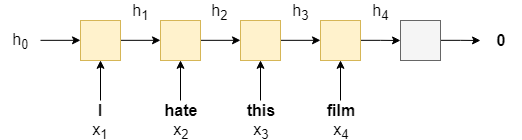
\includegraphics[width=0.9\textwidth]{report-data/rnn.png}
    \caption{RNN}
\end{figure}

RNN 以1个词$x$和一个隐藏状态$h_0$作为输入,并产生下一个隐藏状态$h$。我们对词序列$X=\{x_1,\ldots,x_T\}$循环使用 RNN,将当前词$x_t$以及前一个隐藏状态$h_{t-1}$作为输入,产生隐藏状态$h_t$,即

\begin{equation}
    h_t=\textrm{RNN}(x_t,h_{t-1})
\end{equation}

最后一个隐藏状态$h_t$经过一个全连接层后即可得到预测值。

RNN有多个变种,如双向RNN:

\begin{figure}[H]
    \centering
    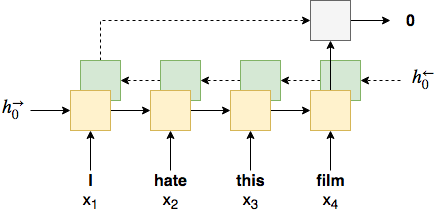
\includegraphics[width=0.9\textwidth]{report-data/bi-rnn.png}
    \caption{双向RNN}
\end{figure}

多层RNN:

\begin{figure}[H]
    \centering
    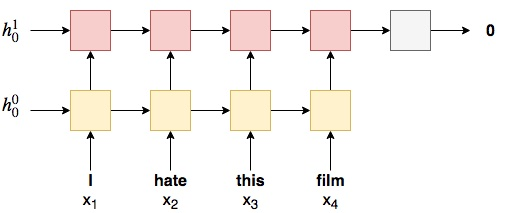
\includegraphics[width=0.9\textwidth]{report-data/mul-rnn.jpg}
    \caption{多层RNN}
\end{figure}

标准的RNN有梯度消失的问题。我们使用如下图所示的LSTM解决此问题:

\begin{figure}[H]
    \centering
    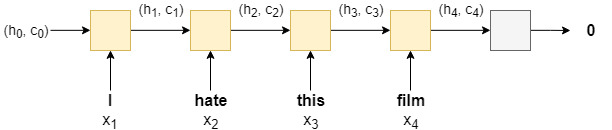
\includegraphics[width=0.9\textwidth]{report-data/lstm.png}
    \caption{LSTM}
\end{figure}

与标准RNN相比,LSTM多了一个额外的状态$c$:

\begin{equation}
    (h_t,c_t)=\textrm{LSTM}(x_t,h_{t-1},c_{t-1})
\end{equation}

LSTM使用多个门控制信息流入和流出$c$,以达到“记忆”的功能。

\begin{figure}[H]
    \centering
    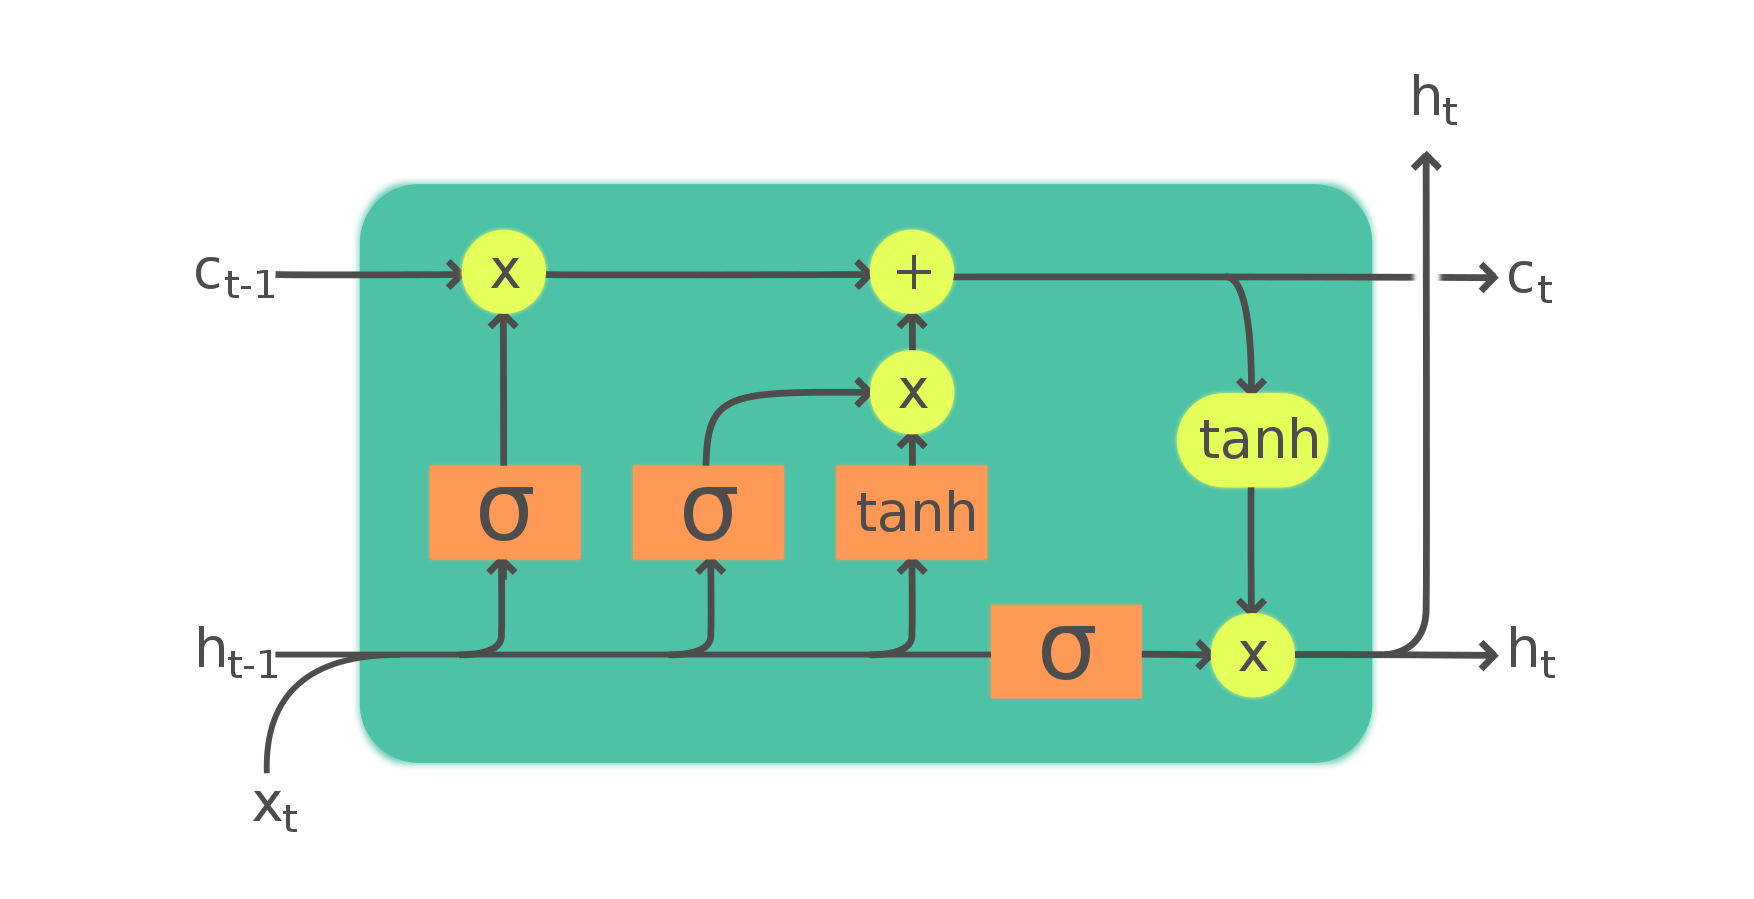
\includegraphics[width=0.9\textwidth]{report-data/lstm-cell.png}
    \caption{LSTM cell}
\end{figure}

\subsection{CNN}

将词向量纵向排列,得到一个二维的输入。

\begin{figure}[H]
    \centering
    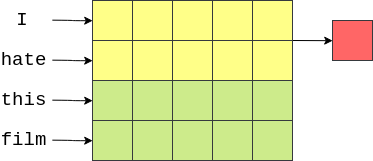
\includegraphics[width=0.9\textwidth]{report-data/cnn-1.png}
    \caption{卷积层}
\end{figure}

输入经过卷积层后得到一个一维的向量。我们对其进行最大池化,即可得到结果:

\begin{figure}[H]
    \centering
    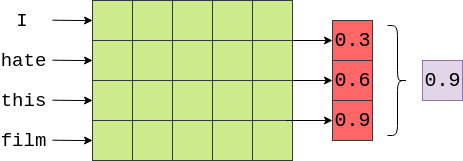
\includegraphics[width=0.9\textwidth]{report-data/cnn-2.png}
    \caption{最大池化}
\end{figure}

为了提取不同长度的词的组合的特征(如“非常 好”和“非常”“好”),我们使用多个大小(如1,2,3)的卷积核,并将进行最大池化的结果拼接在一起,通过全连接层产生输出。

\section{实验结果}



\end{document}
